\chapter{Theoretical Background}\label{ch:2}
\begin{multicols}{2}

There are several different ways in which a variational approach to modelling SMAs can be taken. Generally, the models discussed here fall under the umbrella of `Homogenized Energy Models' as described in \cite{smith2005smart}. The basic idea is to balance the ``the Gibbs and thermal energies through Boltzmann [thermodynamic] principles in single crystal compounds." The homogenization refers to the fact that the theory begins with relations describing the material at the lattice-level (or mesoscale), and is then integrated over a distribution to yield a macroscopic model. Particularly, as Smith explains, ``lattice variations, polycrystallinity, and variable stresses are subsequently incorporated by assuming that parameters such as relative and effective stresses are manifestations of underlying distributions rather than constants" \cite{smith2005smart}\footnote{\textit{Polycrystallinity} refers to the presence of crystal structures in varying orientations in the bulk of the material.}. Meaning these values are functions of model parameters such as $T$ or $\varepsilon$ (see section \ref{sec:HEM}). Thus, the model at once incorporates both micro- and macroscopic features to effectively simulate the material behaviour. 

\section{Thermodynamic Energy Relations} 
Here we present a homogenization approach for uniaxial SMA behaviour. As mentioned, a driving principle is the balancing of Gibbs and Helmholtz energies. The Gibbs free energy is given by
\begin{equation}
    G(\sigma, \varepsilon, T) = \psi(\varepsilon, T) - \sigma\varepsilon, \label{eq:01}
\end{equation}
where $\psi(\varepsilon, T)$ is the Helmholtz energy, $T$ is the temperature, and $\varepsilon$ is the uniaxial shear strain. The equilibrium value for $\varepsilon$ is $\varepsilon = 0$ for austenite and $\varepsilon = \varepsilon_T$ for detwinned martensite in the absence of external stress. As seen in figure \ref{fig:phases} (c), the detwinned martensite possesses some shear strain by default, whether positive or negative \cite{smith2005smart}.

There exist a number of choices for $\psi(\varepsilon, T)$ depending on the features and level of detail that the model seeks to capture. The trade-off for higher accuracy is of course an increased number of undetermined parameters and hence a greater computational challenge. The lowest-order polynomial expansion that exhibits first-order phase transitions,\footnote{In the Ehrenfest classification system, phase transitions are labeled by the lowest order derivative for which the free energy is discontinuous \cite{blundell2010concepts}. (i.e. the first derivative of $\psi$ is discontinuous for $1^{st}$-order phase transition such as solid to liquid.)} is the sixth-degree Falk polynomial,
\begin{equation} \label{eq:02}
    \psi(\varepsilon, T) = \psi_0(T) + \alpha_1(T - T_0)\varepsilon^2 - \alpha_2\varepsilon^4 + \alpha_3\varepsilon^6,
\end{equation}
where $\alpha_1, \alpha_2, \alpha_3$  are positive constants and $T_0$ is the Curie temperature (the point above which the SMA loses its permanent magnetic properties). Typically, the first term is taken to be $\psi_0(T) = -TS$ where $S$ is the specific entropy. $\psi$ can also be defined as a higher order polynomial expansion or a piecewise $C^1$ function.

Equivalent to the second law of thermodynamics, the principle of minimum energy states that a closed system with a fixed entropy will minimize the total energy at equilibrium \cite{callen1985thermodynamics}. Consequently, at a given temperature and external stress, the material strains will react such that $G(\sigma, \varepsilon, T)$ is minimized. Necessary conditions for the minimization of $G$ are
\begin{equation} \label{eq:G_cond1}
    \frac{\partial G}{\partial \varepsilon} = 0, \quad \frac{\partial^2 G}{\partial\varepsilon^2} > 0,
\end{equation}
the first of which implies
\begin{equation} \label{eq:psi_cond}
    \frac{\partial \psi}{\partial \varepsilon} = \sigma,
\end{equation}
by equation (\ref{eq:01}). Accordingly, one can obtain a constitutive relation between the stress $\sigma$ and the shear strain $\varepsilon$ by differentiating (\ref{eq:02}) and setting it equal to $\sigma$. This relation can then be used to draw a predicted stress-strain curve. For examples at different temperatures, see figure \ref{fig:Psi_curves} below.

It is worth noting that the second condition in (\ref{eq:G_cond1}) implies that $G$ is strictly convex, meaning the material will achieve a unique minimizing state at equilibrium. 

\begin{figure}[H]
    \centering
    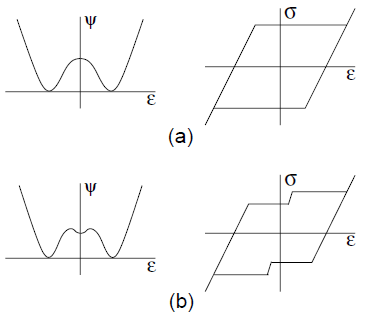
\includegraphics[scale=0.50]{._figures/psi_curves (2).png}
    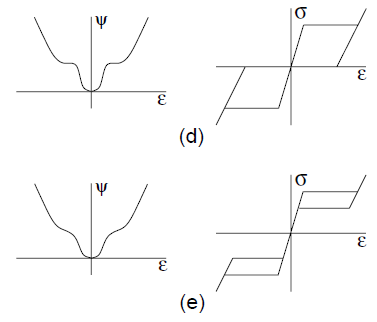
\includegraphics[scale=0.55]{._figures/psi_curves (3).png}
    \caption[Energy density and stress-strain curves]{$\psi$ and $\sigma$-$\varepsilon$ curves given by \ref{eq:G_cond1}-\ref{eq:psi_cond}. (a) $T < T_0$: shape memory effect is observed, in (d) $T = T_1$\footnotemark: pseudoelastic behaviour begins to be observed, (b) and (e) both show intermediate states at lower and higher temperatures respectively \cite{smith2005smart}.}
    \label{fig:Psi_curves}
\end{figure}

\footnotetext{At $T_1 = A_f$ the SMA defaults to the austenite phase, though martensite variants can be induced by sufficiently large stresses.}

Figure \ref{fig:G_curves} shows the Gibbs free energy for a fixed temperature in the austenite regime ($T > A_f$) at $\sigma = 0$ as well as the critical stress values $\sigma_M$, where the transition to martensite begins, and $\sigma_A$ where the reverse process occurs upon unloading. Figure \ref{fig:G_curves} (b) is a plot of the local stress-strain curve for the same temperature (similar to figure \ref{fig:Psi_curves} (e)), neglecting thermal activation ($kT/V$ is small). Finally,  figure \ref{fig:G_curves} (c) shows the stress-strain curve incorporating the effects of thermal activation on the phase transitions, which results in a `smoothing' of the graph at the transition points; closer to what is observed experimentally.

\begin{figure}[H]
    \centering
    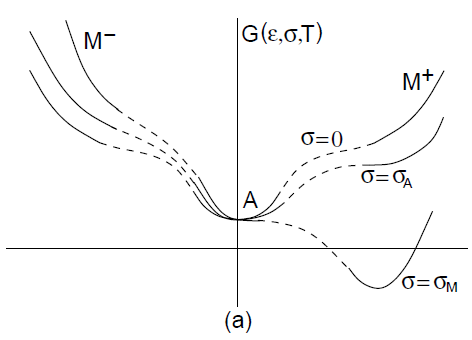
\includegraphics[scale=0.47]{._figures/G_curves_a.png}
\end{figure}

\begin{figure}[H]
    \centering
    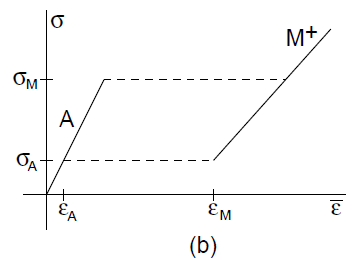
\includegraphics[scale=0.5]{._figures/G_curves_b.png}
    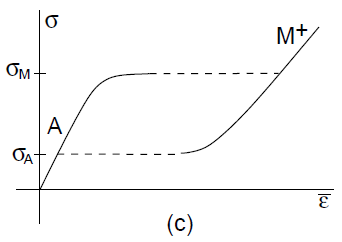
\includegraphics[scale=0.5]{._figures/G_curves_c.png}
    \caption[Gibbs energy and stress-strain curves]{Gibbs energy and stress-strain curves resulting from \ref{eq:01} (a), \ref{eq:G_cond1} (b), and consideration for thermally-activated phase transitions (c). Retrieved from \cite{smith2005smart}.}
    \label{fig:G_curves}
\end{figure}

In order to ``incorporate nonlocal effects such as interfacial energies or domain wall effects," one can augment the Helmholtz energy by the addition of the gradient term $\varepsilon_{x}^2$ \cite{smith2005smart}. The interfacial or surface energy refers to the excess energy present in lattice elements at a surface compared to those in the bulk, due to the surface being less energetically favourable.

\begin{equation} \label{eq:augmented_psi}
    \Tilde{\psi}(\varepsilon,\varepsilon_x,T) = \psi(\varepsilon,T) + \frac{\gamma}{2}\varepsilon_{x}^2.
\end{equation} 

\subsection{Shear Strains of an SMA Rod}
As an illustrative example, we can now consider the case of an SMA rod of length $\ell$ and cross-sectional area $A$, subject to an applied force $f(t,x)$. If $u$ is the longitudinal displacement of the rod, then $\varepsilon$ is related to $u$ by
\begin{equation} \label{eq:u_and_ep}
    \varepsilon(t,x) = \frac{\partial u}{\partial x}(t,x),
\end{equation}
and the total free energy of the system is
\begin{equation} \label{eq:U}
    U(t) = A \bigintsss_0^{\ell} \left[\psi(\varepsilon(t,x),T) + \frac{\gamma}{2}\varepsilon_x^2(t,x) - \rho u(t,x) f(t,x) \right]\mathrm{d}x.
\end{equation}
The kinetic energy is
\begin{equation} \label{eq:K}
    K(t) = A \bigintsss_0^{\ell} \frac{\rho}{2}u_t^2(t,x) \mathrm{d}x.
\end{equation}
The Lagrangian is $\mathcal{L} = K - U$ and the action is
\begin{equation} \label{eq:A}
    \mathcal{A} = \int_a^b\int_0^{\ell} \left(\frac{\rho}{2}u_t^2 - \psi(\varepsilon, T) - \frac{\gamma}{2}\varepsilon_x^2 + \rho u f \right) \mathrm{d}x \mathrm{d}t.
\end{equation}
By Hamilton's principle, the displacement $u$ will make stationary the action. We begin by finding the Gateaux derivative of the action, considering a variation $v(t,x)$. Making the substitution $\varepsilon = u_x$ (by \ref{eq:u_and_ep}),
\begin{equation} \label{eq:A_2}
    \mathcal{A} = \int_a^b\int_0^{\ell} \left(\frac{\rho}{2}u_t^2 - \psi(u_x, T) - \frac{\gamma}{2}u_{xx}^2 + \rho u f \right) \mathrm{d}x \mathrm{d}t.
\end{equation}
Since $\psi$ is a continuous function, $\mathcal{A}(u + \epsilon v)$ is continuous in $\epsilon$ (and is defined for $\epsilon = 0$). Hence, we can compute the variation of $\mathcal{A}$ by taking the derivative,
\begin{align*}
    \delta \mathcal{A}(u;v) &= \frac{\partial \mathcal{A}}{\partial \epsilon}(u + \epsilon v) \biggr\rvert_{\epsilon = 0} \\
    &= \frac{\partial}{\partial\epsilon} \int_a^b \int_0^{\ell} \bigg(\frac{\rho}{2}(u_t + \epsilon v_t)^2 - \psi(u_x + \epsilon v_x, T)\\
    & \quad - \frac{\gamma}{2}(u_{xx} + \epsilon v_{xx})^2 + \rho(u + \epsilon v)f \bigg) \mathrm{d}x \mathrm{d}t \biggr\rvert_{\epsilon = 0}\\
    &= \int_a^b \int_0^{\ell} \bigg(\rho u_t v_t - \frac{\partial\psi}{\partial\varepsilon}(u_x, T)v_x - \gamma u_{xx}v_{xx}\\
    & \qquad + \rho v f \bigg) \mathrm{d}x \mathrm{d}t
\end{align*}
Next, apply integration by parts. We assume that all boundary terms vanish, as they depend on any given boundary values and will simply yield different natural boundary conditions depending on the situation.
\begin{align*}
    \delta \mathcal{A}(u;v) &= \int_0^{\ell}\int_a^b \rho u_tv_t \mathrm{d}t\mathrm{d}x - \int_a^b\int_0^{\ell} \frac{\partial\psi}{\partial\varepsilon}v_x\mathrm{d}x \mathrm{d}t \\
    & \quad \int_a^b\int_0^{\ell}\gamma u_{xx}v_{xx}\mathrm{d}x\mathrm{d}t + \int_a^b\int_0^{\ell}\rho v f\mathrm{d}x\mathrm{d}t \\
    &= \int_0^{\ell} \left(\rho u_tv\biggr\rvert_a^b - \int_a^b \rho u_{tt}v\mathrm{d}t \right) \mathrm{d}x \\
    & \quad - \int_a^b \left(\frac{\partial\psi}{\partial\varepsilon}v\biggr\rvert_0^{\ell} - \int_0^{\ell} \frac{\partial}{\partial x} \left(\frac{\partial\psi}{\partial\varepsilon}\right) v\mathrm{d}x \right)\mathrm{d}t \\ 
    & \quad - \int_a^b \left(\gamma u_{xx}v_{x}\biggr\rvert_0^{\ell} - \int_0^{\ell}\gamma u_{xxx}v_x\mathrm{d}x \right)\mathrm{d}t \\
    & \quad + \int_a^b\int_0^{\ell}\rho v f\mathrm{d}x\mathrm{d}t
\end{align*}
Collecting terms and applying integration by parts with respect to $x$ once again on the third term,
\begin{align*}
    \delta \mathcal{A}(u;v) &= \int_a^b \int_0^{\ell} \left(-\rho u_{tt} + \frac{\partial}{\partial x} \left(\frac{\partial\psi}{\partial\varepsilon}\right) + \rho f \right) v\mathrm{d}x\mathrm{d}t \\
    & \quad + \int_a^b \left(\gamma u_{xxx}v\biggr\rvert_0^{\ell} - \int_0^{\ell}\gamma u_{xxxx}v\mathrm{d}x \right)\mathrm{d}t \\
    &= \int_a^b \int_0^{\ell} \bigg( -\rho u_{tt} + \frac{\partial}{\partial x}\left( \frac{\partial\psi}{\partial\varepsilon}\right) + \rho f\\
    & \quad -\gamma u_{xxxx} \bigg) v(t,x) \mathrm{d}x \mathrm{d}t
\end{align*}
Since the variation $v$ is arbitrary, this means that $u(t,x)$ must satisfy the partial differential equation:
\begin{equation} \label{PDE_u}
    \rho u_{tt} - \frac{\partial}{\partial x}\left(\frac{\partial\psi}{\partial \varepsilon} \right) + \gamma u_{xxxx} = \rho f(t,x)
\end{equation}
where $\psi$ is given by (\ref{eq:02}) or an equivalent Helmholtz energy. Equations which govern the transfer of heat within an SMA sample over time may also be derived. However, these are considerably more complicated than the example given here and are hence not included. 

\subsection{Homogenized Energy Model} \label{sec:HEM}
A common approach taken when considering simple SMA configurations with a high degree of symmetry, such as wires, rods, or thin films, is to treat the sample as being comprised of varying fractions of austenite and martensite phases \cite{smith2005smart}. For simplicity, we consider austenite ($A$) and detwinned martensite ($M^+$, $M^-$) lattice elements. Denote the total volume fractions of $A$, $M^+$, and $M^-$ as $x_A(t)$, $x_+(t)$, and $x_-(t)$ respectively such that $x_A + x_+ + x_- = 1$ at all times. Taking the thermal activation of phase transitions into account, it is possible to develop rate equations for $x_A$, $x_+$, and $x_-$. (See section 5.5.1 in \cite{smith2005smart} for details.) Then, in the case of significant thermal activation, the local average strains are characterized by
\begin{equation} \label{eq:local_strains}
    \Bar{\varepsilon} =  \langle\varepsilon_-\rangle x_- + \langle\varepsilon_+\rangle x_+ + \langle\varepsilon_A\rangle x_A
\end{equation}

As mentioned, to account for material inhomogeneities and lattice variations in going from the mesoscopic to macroscopic model, we treat the relative and effective stresses as distributions. The relative stress is defined as the difference
\begin{equation} \label{eq:rel_st}
    \sigma_R(T) = \sigma_M(T) - \sigma_A(T)
\end{equation}
where the transformation stresses $\sigma_M$ and $\sigma_A$ are those described in section \ref{sec:properties}. Additionally, the effective stress in the material, $\sigma_e$ is the combination of the applied stress and stresses due to local interactions in the lattice, $\sigma_I$.
\begin{equation} \label{eq:eff_st}
    \sigma_e = \sigma + \sigma_I
\end{equation}
To characterize the non-constant nature of $\sigma_R$ and $\sigma_e$, we define two underlying densities $\nu_1$ and $\nu_2$. Possible choices for $\nu_1$, $\nu_2$ include:
\begin{equation} \label{eq:nu1}
    \nu_1(\sigma_R) = c_1 e^{-[\ln(\sigma_R/\Bar{\sigma}_R)/2c]^2}
\end{equation}
which accounts for the fact that $\sigma_M \geq \sigma_A$, and so $\sigma_R \geq 0$. For $\nu_2$ we have 
\begin{align} 
    \nu_2(\sigma_I) &= c_2 e^{-\sigma_{I}^{2}/2b^2},\mathrm{\  and}\label{eq:nu2a}\\
    \nu_2(\sigma_I) &= c_2 e^{-|\sigma_I|/b}. \label{eq:nu2b}
\end{align}
Equation (\ref{eq:nu1}) is known as a lognormal distribution, (\ref{eq:nu2a}) is a `normal density', and (\ref{eq:nu2b}) is called a Laplace relation. Alternatively, $\nu_1$ and $\nu_2$ can be taken as general densities that satisfy the following conditions:
\begin{enumerate}[(i)]
    \item $\nu_1(x)$ is defined for $x > 0$ \quad (\textit{positivity})
    \item $\nu_2(-x) = \nu_2(x)$ \quad (\textit{symmetry})\label{eq:symmetry}
    \item $\smash{\abs{\nu_1(x)} \leq c_1 e^{-a_1 x},\ \abs{\nu_2(x)} \leq c_2 e^{-a_2 x}}$ (\textit{integrability})
\end{enumerate}
Where $c_1$, $a_1$, $c_2$, $a_2 > 0$. Then, the time evolution of the bulk strains as a function of the input stress and temperature (these can be thought of as control variables) is governed by:
\begin{equation*} \label{eq:bulk_strain}
    \resizebox{0.48\textwidth}{!}{\smash{\varepsilon(\sigma,T;t) = \bigintss_{0}^{\infty}\hspace{-.7em} \bigintss_{-\infty}^{\infty} \nu_1(\sigma_R) \nu_2(\sigma_I)\\ \Bar{\varepsilon}(\sigma + \sigma_I, T; \sigma_R, t) \mathrm{d}\sigma_I \mathrm{d}\sigma_R}}
\end{equation*}
meaning we have arrived at a macroscopic relation descibing the stress-strain behaviour of the material subject to external stress $\sigma$ and temperature $T$ (which can depend on time). The function $\Bar{\varepsilon}$ is as defined in equation (\ref{eq:local_strains}).

\section{Entropy Gradient Flow}
Auricchio et al. \cite{auricchio2016gradient}, cast the problem as a generalized gradient flow of the total entropy, $S(\mathbf{y})$. This means that the system state satisfies,
\begin{equation} \label{eq:1}
   \frac{\partial K(t, \mathbf{y}, \mathbf{\dot{y}})}{\partial \mathbf{\dot{y}}} -  \nabla S = 0
\end{equation}
in the case of smooth $K$ and $S$. $K$ is defined as the \textit{entropy production potential} and satisfies the condition: for all $(t, \mathbf{y})$, $\mathbf{\dot{y}} \mapsto K(t, \mathbf{y}, \mathbf{\dot{y}})$ is convex, non-negative, and $K(t, \mathbf{y}, \mathbf{0}) = 0$.

The approach taken here is based upon the General Equations for Non-Equilibrium Reversible-Irreversible Coupling (GENERIC) formalism for thermodynamic systems. The theory is specifically tailored to systems with both reversible and irreversible dynamics, including the hysteretic behaviour exhibited by SMAs \cite{auricchio2016gradient}. Generally speaking, reversible processes relate to changes in free-energy, while irreversible processes relate to changes in entropy (as per the second law of thermodynamics).

\subsection{Notation \& Definitions}
To model three-dimensional stresses and strains, it is necessary to make use of tensors. In keeping with \cite{auricchio2016gradient}, bold letters denote vectors and 2-tensors (which can be expressed as matrices) and double capital letters represent 4-tensors. 4-tensors can be thought of as higher-dimensional arrays with four indices. Given matrices $\bm{\alpha}, \bm{\beta} \in \mathbb{R}^{3\times3}$ and the tensor $\mathbb{A} \in \mathbb{R}^{3\times3\times3\times3}$, define the scalar product $\bm{\alpha} : \bm{\beta} \in \mathbb{R}$ as 

$$\bm{\alpha} : \bm{\beta} \equiv \alpha_{ij}\beta_{ij}$$

and the product $\mathbb{A}\bm{\beta} \in \mathbb{R}^{3\times3}$ as\footnote{These definitions make use of the Einstein summation convention: any repeated index in the expression is summed over, i.e. $\alpha_{ij}\beta_{ij} := \sum_{i=1}^{3}\sum_{j=1}^{3} \alpha_{ij}\beta_{ij}$}

$$(\mathbb{A}\bm{\beta})_{ij} \equiv A_{ijlk}\beta_{lk}$$

A majority of the tensors used here are symmetric, hence $\mathbb{R}^{3\times3}_{\mathrm{sym}}$ is used to refer to the set of $3\times3$ symmetric 2-tensors. The trace is defined in the usual way, $\mathrm{tr}(\bm{\alpha}) = \alpha_{ii}$. Consistent with the earlier definition of the scalar product, the natural inner product for real, square matrices is

$$\bm{\alpha}:\bm{\beta} \equiv \mathrm{tr}(\bm{\alpha}\bm{\beta}^T) = \mathrm{tr}(\bm{\alpha}\bm{\beta})$$

since $\bm{\beta}$ is symmetric. This defines the scalar product on $\mathbb{R}^{3\times3}_{\mathrm{sym}}$, with the corresponding norm $|\bm{\alpha}|^2 = \bm{\alpha}:\bm{\alpha}$. Finally, an important subspace of $\mathbb{R}^{3\times3}_{\mathrm{sym}}$ is the set of \textit{deviatoric} symmetric matrices, $\mathbb{R}^{3\times3}_{\mathrm{dev}}$ given by $\{\alpha \in \mathbb{R}^{3\times3}_{\mathrm{sym}}|\mathrm{tr}(\alpha) = 0\}$. Any symmetric matrix can then be decomposed into $\bm{\alpha} = \mathrm{dev}(\bm{\alpha}) + \frac{1}{3}\mathrm{tr}(\bm{\alpha})\mathbb{I}$ where $\mathrm{dev}(\bm{\alpha})$ is given by:
$$\mathrm{dev}(\bm{\alpha})=\begin{pmatrix}
\alpha_{11} - \tau & \alpha_{12} & \alpha_{13}\\
\alpha_{21} & \alpha_{22} - \tau & \alpha_{23}\\
\alpha_{31} & \alpha_{32} & \alpha_{33} - \tau
\end{pmatrix}$$
with $\tau = \frac{1}{3}\mathrm{tr}(\bm{\alpha})$.

\subsection{Free-Energy Density}\label{sec:FED}
Define $\mathbf{u}: \Omega \longrightarrow \mathbb{R}^3$ to be the displacement from the reference configuration of the sample, $\Omega \subset \mathbb{R}^3$. In the small-deformation regime, decompose the linearized strain,
\begin{equation} \label{eq:2}
    \bm{\varepsilon}(\mathbf{u}) = \frac{1}{2}(\nabla\mathbf{u} + \nabla\mathbf{u}^{T}) 
\end{equation}
as
\begin{equation} \label{eq:3}
    \bm{\varepsilon} = \bm{\varepsilon}^{el} + \mathbf{e}^{tr}
\end{equation}
 where $\bm{\varepsilon}^{el}$ is the elastic component of the strain and $\mathbf{e}^{tr}$ is the inelastic strain associated with transformation and reorientation of the martensitic domains. Particularly, $\mathbf{e}^{tr}$ acts as an internal variable to characterize the phase composition analogous to $x_\pm$ described in section \ref{sec:HEM} \cite{smith2005smart}. The value $|\mathbf{e}^{tr}|$ is then a measure of the martensitic content of the sample, which satisfies $|\mathbf{e}^{tr}| \leq \epsilon_L$ (where $\epsilon_L$ is the maximum strain that can occur due to martensitic reorientation) \cite{auricchio2016gradient}. As the process is assumed to be isochoric, $\mathbf{e}^{tr}$ can therefore be assumed to be deviatoric.

The equilibrium of the Shape Memory Alloy is described by the free-energy density which can be defined as follows:

\begin{multline}
\psi(\bm{\varepsilon}, \mathbf{e}^{tr}, T) = cT(1 - \log T) + \frac{1}{2}(\bm{\varepsilon} - \mathbf{e}^{tr}):\mathbb{C}(\bm{\varepsilon} - \mathbf{e}^{tr})\\
 + \frac{H}{2}|\mathbf{e}^{tr}|^{2} + f( T)|\mathbf{e}^{tr}| + \mathscr{I}(\mathbf{e}^{tr})\label{eq:freeenergy}
\end{multline}  

where $T$ is the temperature, which is assumed to be uniform for simplicity. Since $f( T)$ is the only term that depends on the temperature, this term encapsulates the thermomechanical coupling of the system. $\mathbb{C}$ is the isotropic elasticity tensor, which relates the stress and the elastic component of the strain via $\bm{\varepsilon}^{el} = \mathbb{C}^{-1}\bm{\sigma}$. The constant $c > 0$ is the specific heat capacity of the sample. $H$ is a hardening parameter, associated with the elastic response of austenite and martensite (assumed to be the same for both variants). Finally, the indicator function $\mathscr{I}:\mathbb{R}_{\mathrm{dev}}^{3\times3} \rightarrow [0,\infty]$ defined as

\begin{align}
    \mathscr{I}(\et) &=
    \begin{cases}
        0 & \text{if $|\mathbf{e}^{tr}| \leq \epsilon_L$} \\
        \infty & \text{otherwise}
    \end{cases}\label{eq:indicator}
\end{align}

serves to enforce the constraint that $|\mathbf{e}^{tr}| \leq \epsilon_L$ for finite energies. Seeing as $\mathbf{e}^{tr}$ is deviatoric, it can be convenient to re-express the free-energy in terms of the volumetric and deviatoric strains. That is, instead of (\ref{eq:3}), decompose the strain as

\begin{equation} \label{eq:5}
    \bm{\varepsilon} = \left(\frac{v}{3}\right)\mathbb{I} + \mathbf{e}
\end{equation}

Here, $v = \mathrm{tr}(\bm{\varepsilon})$ represents the volumetric strain, $\mathbf{e} = \mathrm{dev}(\bm{\varepsilon})$ is the deviatoric strain, and $\mathbb{I}$ is the identity 2-tensor. 

Then, (\ref{eq:freeenergy}) becomes
\begin{multline} \label{eq:6}
    \psi(v, \mathbf{e}, \mathbf{e}^{tr},  T) = c T(1 - \log T) + \frac{K}{2}v^{2} + G|\mathbf{e} - \mathbf{e}^{tr}|^{2}\\
    + \frac{H}{2}|\mathbf{e}^{tr}|^{2} + f( T)|\mathbf{e}^{tr}| + \mathscr{I}(\mathbf{e}^{tr})
\end{multline}

$K, G > 0$ are the bulk modulus and shear modulus, respectively. Suppose $\Omega \subset \mathbb{R}^3$ is the volume occupied by the sample. Then, the total free energy is given by

\begin{equation}
    \Psi(v, \mathbf{e}, \mathbf{e}^{tr},  T) = \int_{\Omega} \psi(v, \mathbf{e}, \mathbf{e}^{tr},  T) \mathrm{d}V
\end{equation}

The constitutive relations which govern the response of the material are then given by the variations of $\psi$ with respect to its variables. Seeing as $\psi$ is rate-independent, the second term of the Euler-Lagrange equation vanishes and the variation reduces to partial differentiation. For a given coordinate $q$,\footnote{$q = \{v, \mathbf{e}, \mathbf{e}^{tr},  T\}$}

\begin{align} \label{eq:7}
    \delta\psi &= \frac{\partial\psi}{\partial q} - \frac{d}{dt}\frac{\partial\psi}{\partial\dot{q}}\\
    \delta\psi &= \frac{\partial\psi}{\partial q}
\end{align}

Using equation (\ref{eq:6}), we obtain the four constitutive relations:

\begin{align}\label{eq:8}
    \frac{\partial\psi}{\partial v} &= Kv \equiv p\\
    \frac{\partial\psi}{\partial\mathbf{e}} &= 2G(\mathbf{e} - \mathbf{e}^{tr}) \equiv \bm{S}_{\mathrm{dev}}\\
    \frac{\partial\psi}{\partial T} &= -c\log{ T} + f'( T)|\mathbf{e}^{tr}| \equiv -s \label{eq:ent}\\
    \frac{\partial\psi}{\partial\mathbf{e}^{tr}} &= -\bm{S}_{\mathrm{dev}} + H\mathbf{e}^{tr} + f(T)\partial|\mathbf{e}^{tr}|\\
    & \quad + \partial \mathscr{I}(\mathbf{e}^{tr}) \quad \quad \qquad \equiv -\bm{X}\nonumber
\end{align}

Here, $p$ is the pressure, $\bm{S}_{\mathrm{dev}}$ is the deviatoric stress, $s$ is the entropy density, and $\bm{X}$ is a thermodynamic variable associated with the internal variable $\mathbf{e}^{tr}$. The Cauchy Stress tensor can then be written as: $\bm{\sigma} = p\mathbb{I} + \bm{S}_{\mathrm{dev}}$ \cite{auricchio2016gradient}. The derivatives of $|\mathbf{e}^{tr}|$ and $I$ are defined as follows:

\begin{align}\begin{split}
    \partial|\mathbf{e}^{tr}| &=
    \begin{cases}
        \frac{\mathbf{e}^{tr}}{|\mathbf{e}^{tr}|} & \text{if $\mathbf{e}^{tr} \neq \bm{0}$}\\
        \bm{0} & \text{if $\mathbf{e}^{tr} = \bm{0}$}
    \end{cases}\\
    \partial \mathscr{I}(\mathbf{e}^{tr}) &=
    \begin{cases}
        \bm{0} & \text{if $|\mathbf{e}^{tr}| < \epsilon_L$}\\
        \xi\frac{\mathbf{e}^{tr}}{|\mathbf{e}^{tr}|}, \xi \geq 0 & \text{if $|\mathbf{e}^{tr}| = \epsilon_L$}\\
        \varnothing & \text{if $|\mathbf{e}^{tr}| > \epsilon_L$}
    \end{cases}
    \end{split}\label{eq:derivative2}
\end{align}

We are now in a position to formulate the entropy as a functional. If we take $\mathbf{y} = (\mathbf{e}^{tr},  T)$ then by (\ref{eq:ent}), the total entropy is:

\begin{equation} \label{eq:9}
    S(\mathbf{y}) = \int_{\Omega} s(\mathbf{y})\mathrm{d}x = \int_{\Omega}(c\log T - f'( T)|\mathbf{e}^{tr}|)\mathrm{d}x
\end{equation}
and the gradient is
\begin{align} \label{eq:10}
    \nabla S &= 
        \begin{pmatrix}
        -f'(T)\partial |\mathbf{e}^{tr}| \\
        c/T - f''( T)|\mathbf{e}^{tr}|
        \end{pmatrix}
\end{align}

This can then be used to determine the system state via equation (\ref{eq:1}). For more details and suitable choices of $K$ and $f$ the reader is referred to \cite{auricchio2016gradient}. 

\section{Extension to Modelling Magnetic SMAs}

\subsection{Defining the Energy Functional}

An interesting class of SMAs are the so called \textit{Magnetic} SMAs (MSMAs). These are materials that can undergo heavy and reversible strains when subjected to an external magnetic field. Among the various MSMAs, the most widely studied is the NiMnGa alloy \cite{webster1984magnetic, ullakko1996large, tickle1999magnetic}. Methods from variational calculus can be used to study these materials and it is the purpose of this section to give an example of how this works.

As in the case of standard SMAs, the system of equations that describe MSMAs can be derived by taking variational derivatives of an energy functional. The MSMA sample is set up such that it is in a single state before an external magnetic field is applied to it. Once the magnetic field is applied, the MSMA undergoes a transformation between two martensitic variant states, hereby called ``variant 1" and ``variant 2" with volume fraction $(1-\xi)$ and $\xi$, respectively. It is also worth pointing out that associated with each of these two variant states, there are two kinds of magnetic domains with respective volume fractions $(1-\alpha)$ and $\alpha$. 

The effective magnetization at a single point inside the MSMA can be defined as
\begin{equation} \label{eq:11}
    \overline{\textbf{M}} = M_{s}\left[(1-\xi)\sin\theta + \xi(2\alpha -1)\right]\textbf{e}_{2}
\end{equation}
where $\textbf{e}_{2}$ is a unit vector along the y-axis and $\theta$ is the angle with which the magentization vector of the material rotates after the application of an external magnetic field. The magnetization of the MSMA will induce the distribution of a magnetic scalar potential $\Psi(\textbf{X})$ in $\mathbb{R}^{3}$ \cite{wang2012variational}.

Following \cite{wang2012variational}, we first will define each term of the energy functional, before putting it all together.

First, the \textit{elastic potential energy} is defined as
\begin{equation} \label{eq:12}
    \mathcal{F}_{el} = \int_{\Omega_{r}}\rho_{r}\phi(\mathbb{F}, \xi)dV
\end{equation}
where $\Omega_{r} \subset \mathbb{R}^{3}$ is the region that the MSMA occupies, $\phi$ is the elastic energy per unit mass, $\rho_{r}$ is the density of the material, and $\mathbb{F}$ is called the deformation gradient tensor. ($\mathbb{F}$ is related to the displacement $\mathbf{u}$ by $\mathbb{F} = \mathbb{I} + \frac{\partial\mathbf{u}}{\partial\mathbf{X}}$, where $\mathbf{X}$ denotes the reference configuration of the sample).

The \textit{magnetocrystalline anisotropy energy} is defined as
\begin{equation} \label{eq:13}
    \mathcal{F}_{an} = \int_{\Omega_{r}} \left(1-\xi\right)\rho_{r}K_{u}\sin^{2}\theta dV
\end{equation}
where $K_{u}$ is called the \textit{anisotropy constant}.

The \textit{Zeeman energy} is
\begin{equation} \label{eq:14}
    \mathcal{F}_{ze} = \int_{\Omega_{r}} -\mu_{0}\rho_{r}\overline{\textbf{M}} \cdot \textbf{H}_{a} dV
\end{equation}
where $\textbf{H}_{a}$ is the external magnetic field and $\overline{\textbf{M}}$ is the magnetization vector defined in (\ref{eq:11}).

The \textit{magnetostatic energy} is
\begin{equation} \label{eq:15}
    \mathcal{F}_\mathrm{sta} = \int_{\Omega_{r}}-\mu_{0}\rho_{r}\overline{\textbf{M}} \cdot \textbf{H}_{d} dV + \int_{\mathbb{R}^{3}}-\frac{\mu_{0}}{2} J \textbf{H}_{d}\cdot \textbf{H}_{d} dV
\end{equation}
where $\textbf{H}_{d} = -\mathbb{F}^{-T}  \nabla(\Psi)$ is the \textit{demagnetization field} induced by the magnetization of the MSMA sample and $J = \text{det}(\mathbb{F})$. Here, $\Psi$ is the scalar magnetic potential in $\mathbb{R}^{3}$ induced by the magnetization of the MSMA itself, as mentioned earlier. $\Psi$ is assumed to be a continous function of $X$ and regular at $\infty$.

The \textit{mixture energy}, due to the micro interactions of the different martensitic variants and magnetic domains is
\begin{align} \label{eq:16}
    &\mathcal{F}_{mix} = \int_{\Omega_{r}}\rho_{r}f^{\xi}(\xi)dV \notag \\
    &+ \int_{\Omega_{r}}\rho_{r} \left[(1-\xi)f^{\alpha}\left(\frac{1}{2}\right) + \xi f^{\alpha}(\alpha)\right]dV
\end{align}
where $f^{\xi}(\xi)$ and $f^{\alpha}(\alpha)$ are the energy densities that come from the mixture of the two variant states and the interactions of the different magnetic domains in each variant region.

The \textit{potential energy of mechanical loading} is
\begin{equation} \label{eq:17}
    \mathcal{F}_{ml} = \int_{\partial\Omega_{r}} -\textbf{t}_{A}\cdot \textbf{x} dA
\end{equation}
where $\textbf{t}_{A}$ is the external traction per unit area applied to the MSMA sample.

Finally, one needs to consider energy dissipation during the transformation of the material from variant 1 to variant 2. By assumption, for this model, the total energy dissipations during the transition can be written as
\begin{equation} \label{eq:18}
    \mathcal{F}_\mathrm{dis} = \pm \int_{\Omega_{r}} \int_{\xi_{0}(\textbf{X})}^{\xi(\textbf{X})} \rho_{r}\mathcal{D}^{\pm}d\tau dV
\end{equation}
where $\xi_{0}(\textbf{X})$ and $\xi(\textbf{X})$ are the initial and  final variant state distributions for the MSMA sample. $\mathcal{D}^{\pm}$ are positive functions called the dissipative resistances. For a MSMA transformation from variant 1 to variant 2, we have $\xi_{0}(\textbf{X})\leq\xi(\textbf{X})$ and we take the $``+"$ dissipative resistance function. If the MSMA undergoes a transformation from variant 2 to variant 1, we have $\xi_{0}(\textbf{X}) \geq \xi(\textbf{X})$ and we take the $``-"$ dissipative resistance function.


Adding up (\ref{eq:12}) - (\ref{eq:18}) gives the total energy functional for the MSMA system. It is written explicitly as
\begin{align} \label{eq:19}
    &\mathcal{G}(\textbf{x}, \Psi, \xi, \alpha, \theta ; \textbf{X}) = \int_{\Omega_{r}}\rho_{r}\phi(\mathbb{F}, \xi)dV \notag \\
    &+ \int_{\Omega_{r}} (1-\xi)\rho_{r}\left(K_{u}\sin^{2}\theta + f^{\alpha}\left(\frac{1}{2}\right)\right) dV \notag \\
    &+ \int_{\Omega_{r}}\rho_{r}f^{\xi}(\xi)dV + \int_{\Omega_{r}}\xi\rho_{r}f^{\alpha}(\alpha)dV \notag \\
    &+ \int_{\Omega_{r}}-\mu_{0}\rho_{r}\overline{\textbf{M}} \cdot \textbf{H}_{a} dV + \int_{\Omega_{r}}-\mu_{0}\rho_{r}\overline{\textbf{M}} \cdot \textbf{H}_{d} dV \notag \\
    &+ \int_{\mathbb{R}^{3}}-\frac{\mu_{0}}{2} J \textbf{H}_{d}\cdot \textbf{H}_{d} dV \pm \int_{\Omega} \int_{\xi_{0}(\textbf{X})}^{\xi(\textbf{X})} \rho_{r}\mathcal{D}^{\pm}d\tau dV \notag \\
    &- \int_{\partial\Omega_{r}}\textbf{t}_{A}\cdot \textbf{x} dA
\end{align}
where the independent variables are $\textbf{x}$ and $\Psi$, $\textbf{x}$ being a point inside $\Omega_{r}$. 


\subsection{Governing Equations for MSMAs Using Variational Methods}
This subsection is dedicated to calculating the equations needed to determine the distribution of the scalar potential $\Psi(\textbf{X})$ in $\mathbb{R}^{3}$. We will do this by making use of the calculus of variations and taking the variation of $\mathcal{G}$ in (\ref{eq:18}) with respect to $\Psi$. We will then set this equal to zero, requiring that $\mathcal{G}$ be stationary with respect to $\Psi$. This will naturally lead to two equations that can be used to solve for $\Psi(\textbf{X})$ specific to the MSMA system. This work again comes from \cite{wang2012variational}.

Firstly, the variation of the energy functional $\mathcal{G}$ with respect to the independant variable $\Psi$ is
\begin{align} \label{eq:20}
    \delta_{\Psi}\mathcal{G} &= \delta_{\Psi}\left(\int_{\Omega_{r}}-\mu_{0}\rho_{r}\overline{\textbf{M}} \cdot \textbf{H}_{d} dV\right) \notag \\
    &+ \delta_{\Psi}\left(\int_{\mathbb{R}^{3}}-\frac{\mu_{0}}{2} J \textbf{H}_{d}\cdot \textbf{H}_{d} dV \right) \notag \\
    &=\int_{\Omega_{r}}\mu_{0}\rho_{r}(\mathbb{F}^{-1}\overline{\textbf{M}})\cdot  \nabla(\delta\Psi) dV \notag \\
    &- \int_{\mathbb{R}^{3}}\mu_{0}J(\mathbb{C}^{-1} \nabla\Psi)\cdot  \nabla(\delta\Psi) dV
\end{align}
where $\mathbb{C}$ is defined in equation (\ref{eq:freeenergy}). This is because the terms in (\ref{eq:19}) that contain $\textbf{H}_{d}$ are the only ones that depend on $\Psi$, through the definition of $\textbf{H}_{d}$. One is free to define a ficticious displacement field in a region outside $\Omega_{r}$, which is called $\Omega_{r}^{\prime}$ such that $\textbf{x}$ can be smoothly extended from $\Omega_{r}$ into its exterior \cite{wang2012variational}. Doing this enables the Lagrangian quantities to be defined outside of $\Omega_{r}$. 

Applying the divergence theorem to (\ref{eq:20}) in regions $\Omega_{r}$ and $\Omega_{r}^{\prime}$ yields
\begin{align} \label{eq:21}
    \delta_{\Psi}\mathcal{G} &= -\int_{\Omega_{r}} \nabla\cdot(\textbf{B}_{l})\delta\Psi dV - \int_{\Omega_{r}^{\prime}} \nabla\cdot(\textbf{B}_{l})\delta\Psi dV \notag \\
    &+ \int_{\partial\Omega_{r}}([\textbf{B}_{l}]\cdot \textbf{N})\delta\Psi dS + \int_{\partial\Omega_{\infty}}(\textbf{B}_{l}\cdot\textbf{N})\delta\Psi dS,
\end{align}
where 
\begin{align} \label{eq:22}
    \textbf{B}_{l} &=
    \begin{cases}
        \mu_{0}(\rho_{r}\mathbb{F}^{-1}\overline{\textbf{M}}-J\mathbb{C}^{-1} \nabla\Psi) & \text{in $\Omega_{r}$}\\
        -\mu_{0}J\mathbb{C}^{-1} & \text{in $\Omega_{r}^{\prime}$},
    \end{cases}
\end{align}
and 
\begin{equation} \label{eq:23}
    [\textbf{B}_{l}] = \textbf{B}_{l}^{i} - \textbf{B}_{l}^{o}
\end{equation}
denotes the jump of the enclosed quantity in passing from the outside to the inside of the MSMA sample \cite{wang2012variational}. The last term in (\ref{eq:21}) vanishes because $\textbf{B}_{l} \sim 1/|\textbf{X}|^{2}$ as $|\textbf{X}|\rightarrow\infty$ \cite{wang2012variational}.

Since $\delta\Psi$ is arbitrary, in order for the energy functional $\mathcal{G}$ to be stationary with respect to $\Psi$, we must have

\begin{equation} \label{eq:24}
    \nabla\cdot(\textbf{B}_{l}) = 0
\end{equation}
in $\Omega_{r} \cup \Omega_{r}^{\prime}$ and 
\begin{equation} \label{eq:24}
    [\textbf{B}_{l}] \cdot \textbf{N} = 0
\end{equation}
on $\partial\Omega_{r}$.

These two equations can be used to determine the distribution of the scalar potential $\Psi(\textbf{X})$ in $\mathbb{R}^{3}$. 
































\end{multicols}